\section{Experimental verification}\label{verification}
After reconstructing the dataset by writing dedicated Docker images and ConCap scenarios, we want to experimentally verify that the generated traffic is equivalent.

For the purposes of this dissertation, we define the equivalence of original and synthetic network traffic as follows: a model trained on original traffic can predict synthetic traffic with high degree of accuracy, and vice-versa. 

In their analysis and experiments with CIC-IDS-2017 \cite{distrinet_cic_analysis}, D'Hooge trains a single feature Decision Tree on the entire dataset using usual ML methodology and find ROC AUC scores above .9 for multiple different features. A high imbalance between attack classes and benign samples can be noted: attack traffic accounts for 19.6\% of the total flows presented. 
In this thesis, we follow a methodology similar to theirs to prepare the dataset for testing:
\begin{itemize}
	\item Generate NetFlows from the PCAP files.
	\item Strip metadata columns and clean the dataset by dropping duplicate rows and rows containing NaN values.
\end{itemize}

As class imbalance can lead to skewed results, we want to address it by synthetically augmenting the attack flows with benign traffic. To do this, we separately load and clean the original Monday PCAP file. We call these flows "benign traffic". 

For every attack class, we prepare the two datasets for experiments: the fixed dataset provided by \cite{troubleshooting_cic2017} (the CIC traffic) and the synthetic dataset generated by ConCap (the ConCap traffic). We treat both datasets with the same cleaning procedure as describe above. 

Uing CIC traffic, we train a Decision Tree model with the Gini criterion and a single node, using a single datapoint in the dataset as the decision data point, as done by \cite{distrinet_cic_analysis}. After training, we calculate the model's accuracy of predicting the label of the ConCap traffic. We repeat this procedure in reverse, training on ConCap traffic and evaluating on CIC traffic.


To quantify the performance of the trained models for different features, we calculate following metrics:

\begin{itemize}
	\item \textbf{Recall}: Recall expresses the correctness of model predictions on positive samples as a ratio of true positives with respect to all positive samples: $$ \frac{TP}{TP+FN} $$
	\item \textbf{Accuracy}: a metric expressing the correctness of predictions of a model as a ratio of the correct predictions and total predictions $$\frac{TP + TN}{TP + TN + FN + FP} $$
	\item \textbf{Precision}: Precision describes how precise the model is in its positive predictions, calcualted as a ratio of true positives and all predicted positives: $$ \frac{TP}{TP+FP} $$
	\item \textbf{Area Under Receiver Operator Characteristic Curve (ROC AUC) score}: By calculating the True Positive Rate and False Positive Rate of the model at set intervals, a curve can be plot through them. Area under this curve expresses how the probability of the model predicting a random malicious sample as malicious. 
	
\end{itemize}

The processed NetFlow files can be found on Kaggle\footnote{\url{https://www.kaggle.com/datasets/jozefjankaj/thesis-files}}. We perform the verification experiment for each attack class separately. 

In graphs below, we visualize these metrics for each attack class. Depending on the traffic the model was trained on (either original CIC-IDS-2017 or ConCap scenarios), we find different sets of features that hold most predictive power. We do note that common features can be found in these sets, and suggest that these features are most representative of the underlying traffic. Consequently, it is these common features that should be used as decision features for actual ML-NIDS systems.

\subsection{Tuesday}
\subsubsection{FTP}
For FTP Bruteforce, Figures \ref{fig:ftp_cic_concap} and \ref{fig:ftp_concap_cic} show a range of features performing excellenty, with many scoring above .95 ROC AUC Score. Averaing out the results, we find the top three best performing features for both ways to be Bwd RST Flags (0.978288), Packet Length Mean (0.976290) and Average Packet Size (0.976290).

\begin{figure}[!htbp]
	\centering
	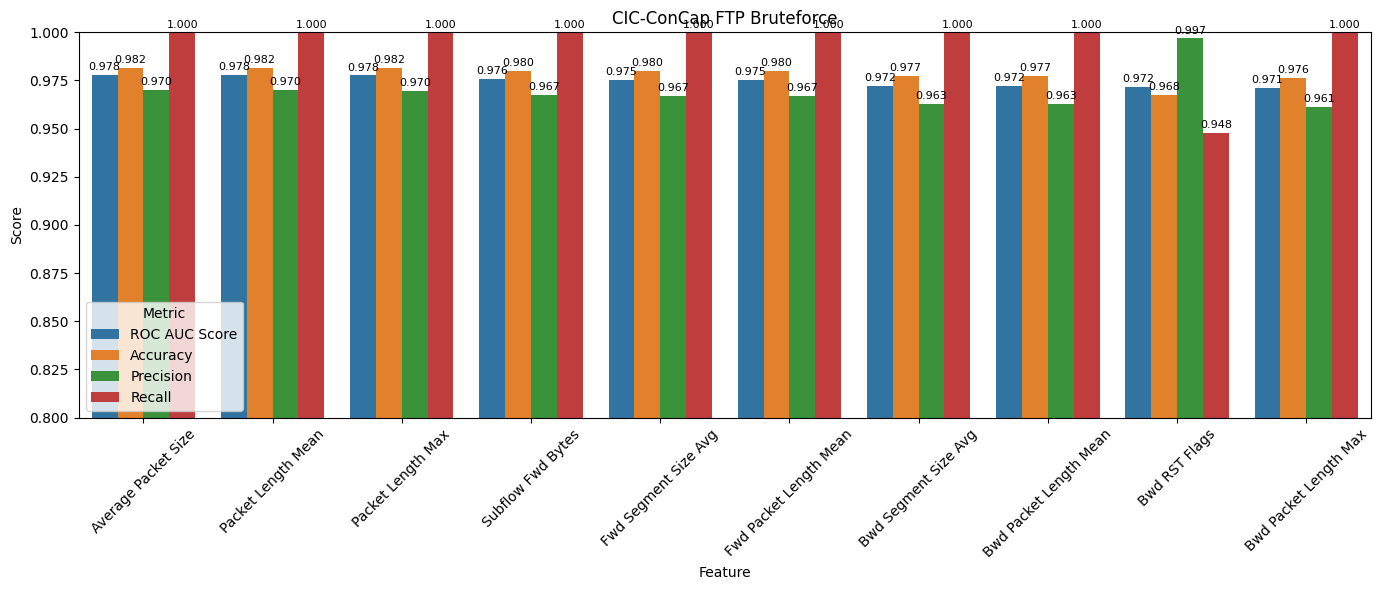
\includegraphics[width=1.2\linewidth]{images/ftp_cic_concap}
	\caption{\\Best performing features for FTP Bruteforce when trained on CIC-IDS-2017 and measured on ConCap traffic}
	\label{fig:ftp_cic_concap}
\end{figure}

\begin{figure}
	\centering
	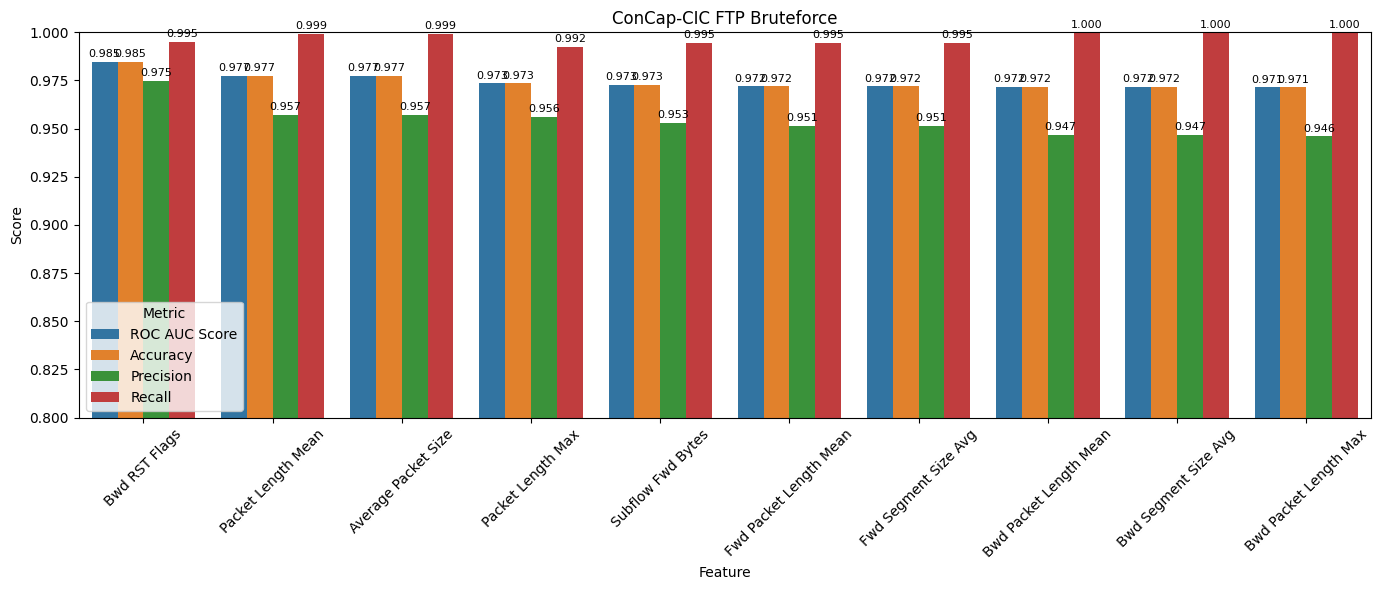
\includegraphics[width=1.2\linewidth]{images/ftp_concap_cic}
	\caption{\\Best performing features for FTP Bruteforce when trained on ConCap traffic and measured on CIC-IDS-2017}
	\label{fig:ftp_concap_cic}
\end{figure}


\subsubsection{SSH}
For SSH Bruteforce, Figures \ref{fig:ssh_cic_concap} and \ref{fig:ssh_concap_cic} show a smaller range of features than FTP Bruteforce, but nonetheless these features maintain a high predictive power. For the top three best performing common features, we find Fwd Seg Size Min (0.922024), Fwd IAT Min (0.854907) and Bwd Segment Size Avg (0.817511). 

\begin{figure}
	\centering
	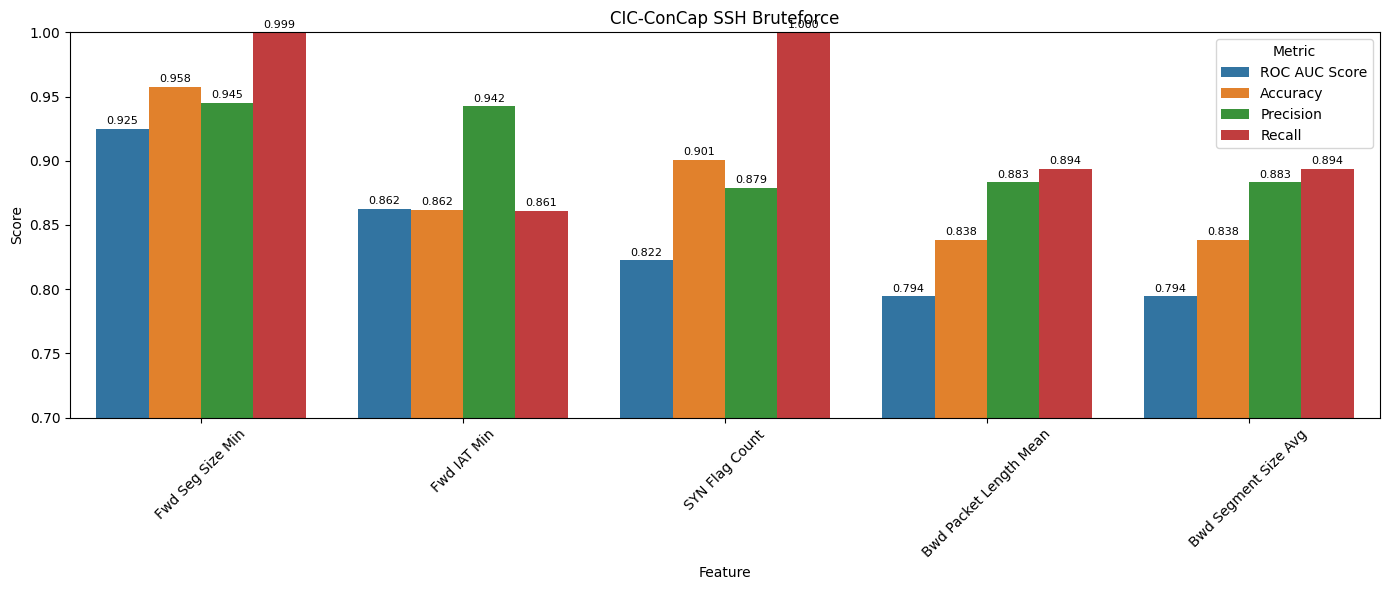
\includegraphics[width=1.2\linewidth]{images/ssh_cic_concap}
	\caption{\\Best performing features for SSH Bruteforce when trained on CIC-IDS-2017 traffic and measured on ConCap traffic}
	\label{fig:ssh_cic_concap}
\end{figure}

\begin{figure}
	\centering
	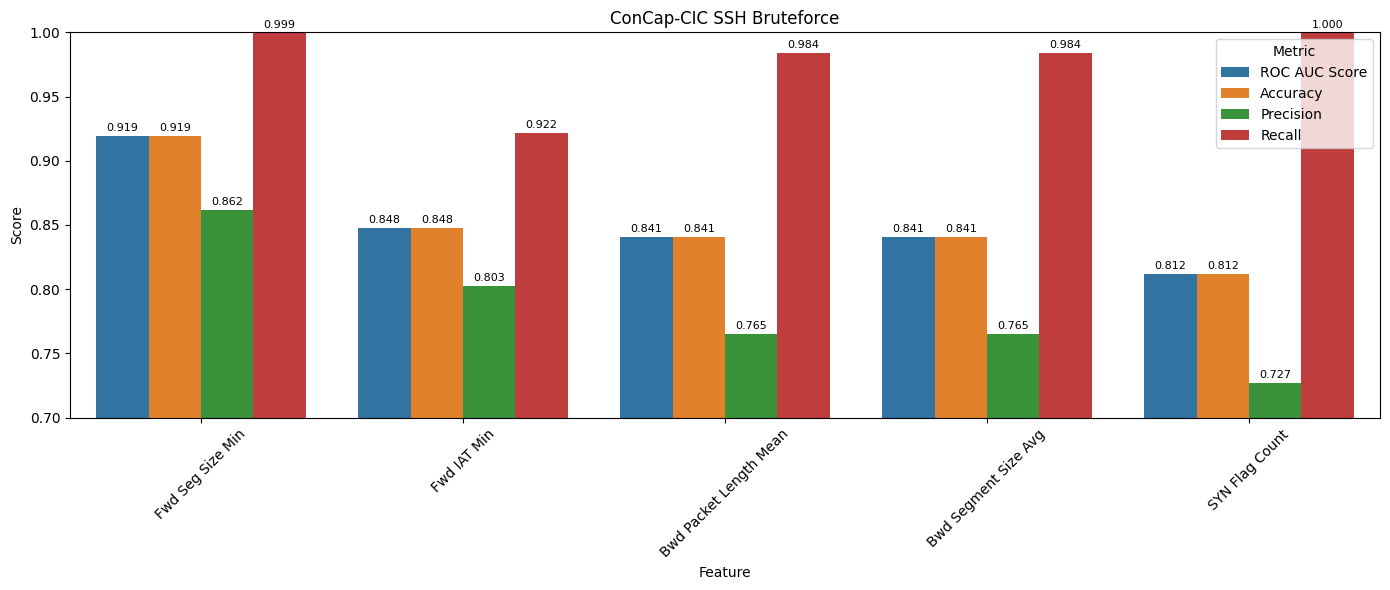
\includegraphics[width=1.2\linewidth]{images/ssh_concap_cic}
	\caption{\\Best performing features for FTP Bruteforce when trained on ConCap traffic and measured on CIC-IDS-2017}
	\label{fig:ssh_concap_cic}
\end{figure}

\FloatBarrier

\subsection{Wednesday}
\subsubsection{Slowloris}
For Slowloris, we mainly find features that focus on flow time and size of packets, as shown by Figures \ref{fig:slowloris_cic_concap} and \ref{fig:slowloris_concap_cic}. Interestingly, we can see that the recall metric for features focused on size plummets when trained on CIC-IDS-2017, suggesting a difference in implementation we were not able to spot. Nonetheless, given the nature of this attack, we expect the main feature with high predictive power to be related to Flow time, and Total TCP Flow Time is precisely that feature. In terms of best common performing features, we find Total TCP Flow Time (0.910773), Bwd Packet Length Max (0.868125) and Total Length of Bwd Packet (0.868125). 

\begin{figure}
	\centering
	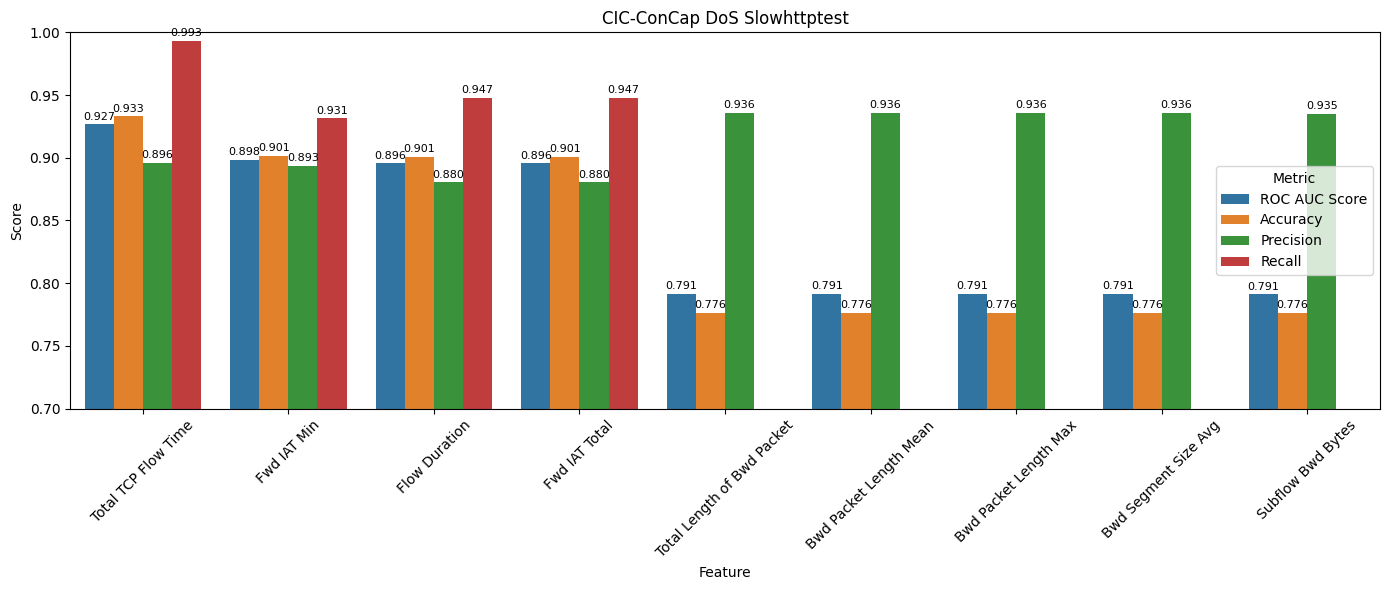
\includegraphics[width=1.2\linewidth]{images/slowhttptest_cic_concap}
	\caption{\\Best performing features for DoS Slowloris when trained on CIC-IDS-2017 traffic and measured on ConCap}
	\label{fig:slowloris_cic_concap}
\end{figure}
\begin{figure}
	\centering
	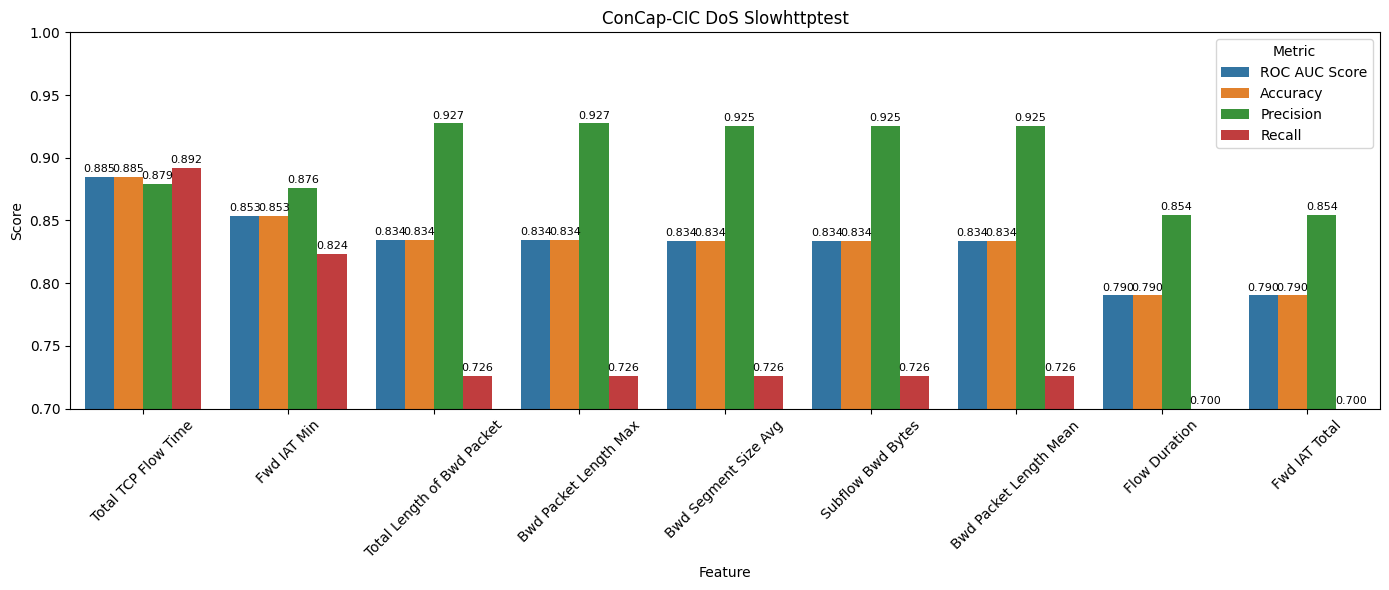
\includegraphics[width=1.2\linewidth]{images/slowhttptest_concap_cic}
	\caption{\\Best performing features for DoS Slowloris when trained on ConCap traffic and measured on CIC-IDS-2017}
	\label{fig:slowloris_concap_cic}
\end{figure}


\subsubsection{Slowhttptest}
Similarly to Slowloris, Figures \ref{fig:slowhttptest_cic_concap} and \ref{fig:slowhttptest_concap_cic} show the Total TCP Flow Time feature to perform best, maintaining high recall and ROC AUC Score. Interestingly, we see far more features that focus on timing than rather than size that we've seen in Slowloris attacks. For the best performing features, we find Total TCP Flow Time (0.905697), Fwd IAT Min (0.875804) and Fwd IAT Total (0.842901).

\begin{figure}
	\centering
	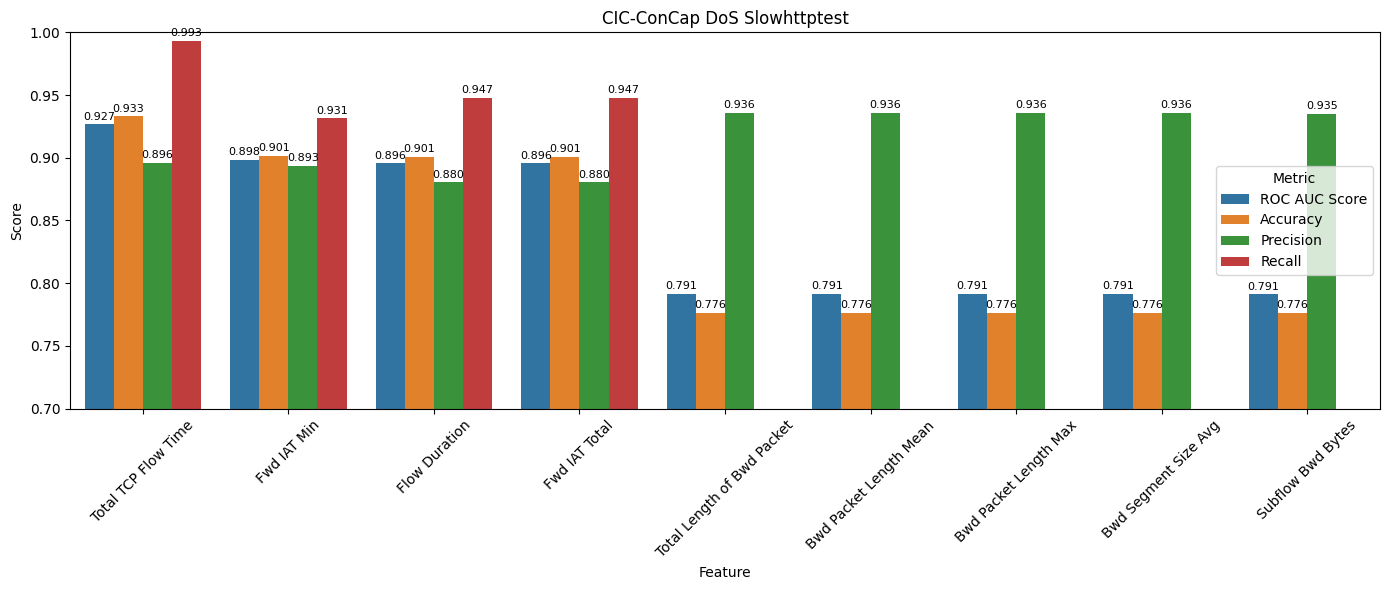
\includegraphics[width=1.2\linewidth]{images/slowhttptest_cic_concap}
	\caption{\\Best performing features for DoS Slowhttptest when trained on ConCap traffic and measured on CIC-IDS-2017}
	\label{fig:slowhttptest_cic_concap}
\end{figure}
\begin{figure}
	\centering
	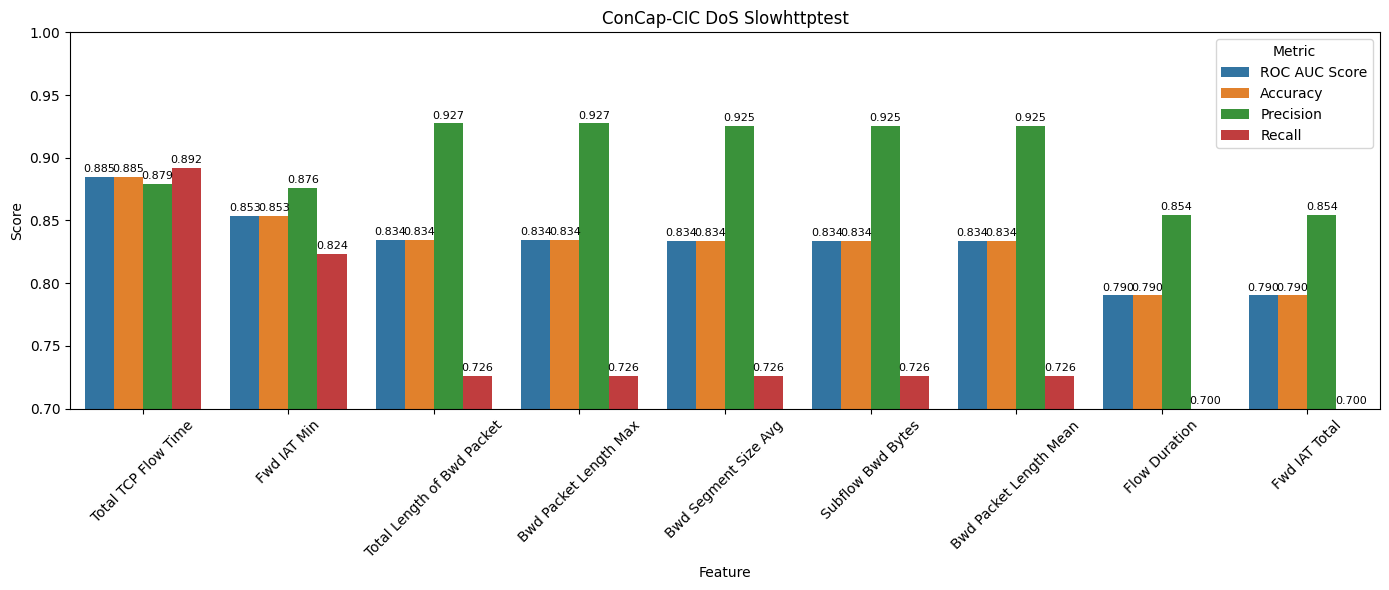
\includegraphics[width=1.2\linewidth]{images/slowhttptest_concap_cic}
	\caption{\\Best performing features for DoS Slowhttptest when trained on ConCap traffic and measured on CIC-IDS-2017}
	\label{fig:slowhttptest_concap_cic}
\end{figure}


\subsubsection{HULK}
For HULK, Figures \ref{fig:hulk_cic_concap} and \ref{fig:hulk_concap_cic} show that mostly features focusing on forward and backward packets hold the most predictive power, performing well across all metrics. For the best performing features, we find Bwd Packet Length Std (0.977942), Fwd RST Flags (0.954837) and Subflow Bwd Bytes (0.951484) to perform best for both ways of testing.


\begin{figure}
	\centering
	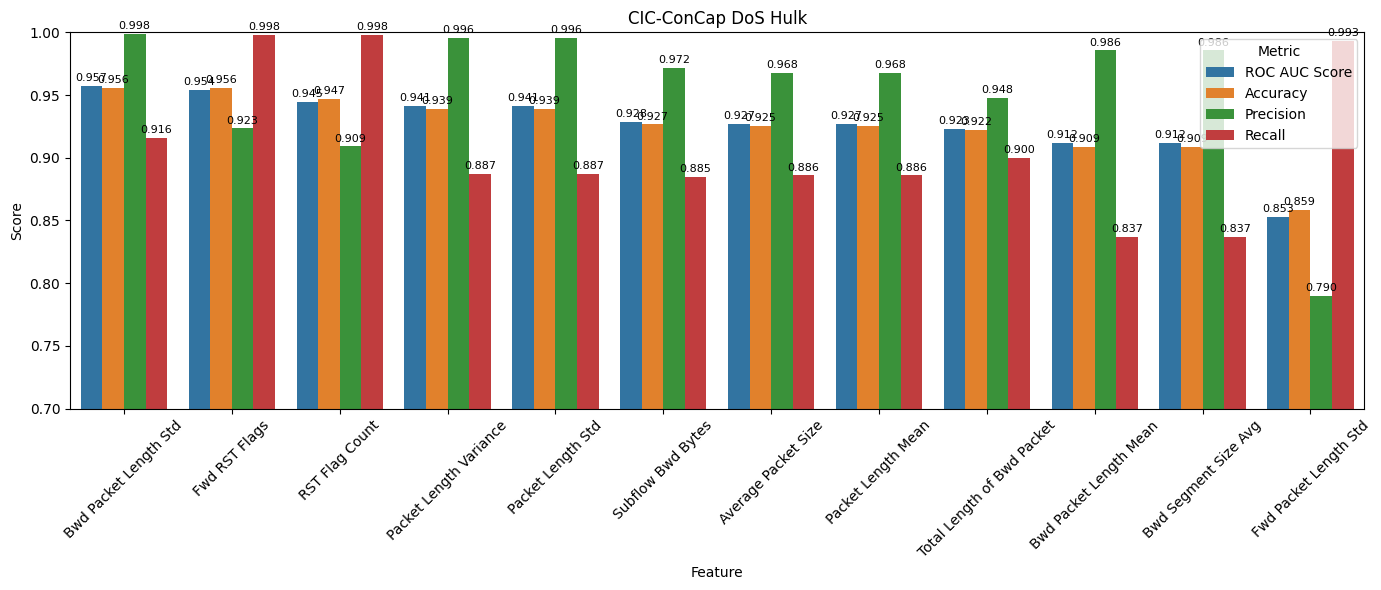
\includegraphics[width=1.2\linewidth]{images/hulk_cic_concap}
	\caption{\\Best performing features for DoS HULK when trained on CIC-IDS-2017 traffic and measured on ConCap}
	\label{fig:hulk_cic_concap}
\end{figure}
\begin{figure}
	\centering
	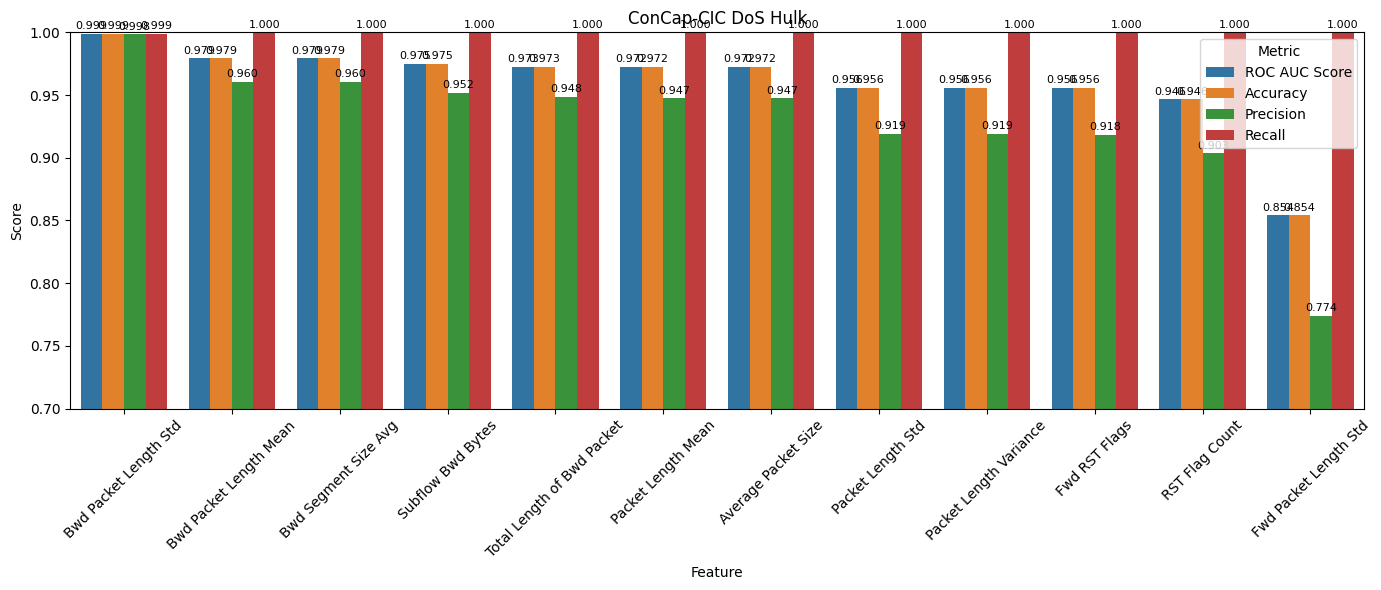
\includegraphics[width=1.2\linewidth]{images/hulk_concap_cic}
	\caption{\\Best performing features for DoS HULK when trained on ConCap traffic and measured on CIC-IDS-2017}
	\label{fig:hulk_concap_cic}
\end{figure}


\subsubsection{GoldenEye}
Figures \ref{fig:goldeneye_cic_concap} and \ref{fig:goldeneye_concap_cic} show a mix of features that predicts GoldenEye attacks well, without a particular focus on any one category. The best performing features are Bwd Packet Length Std (0.939286), Packet Length Variance (0.927954) and Packet Length Std (0.927954). 
\begin{figure}
	\centering
	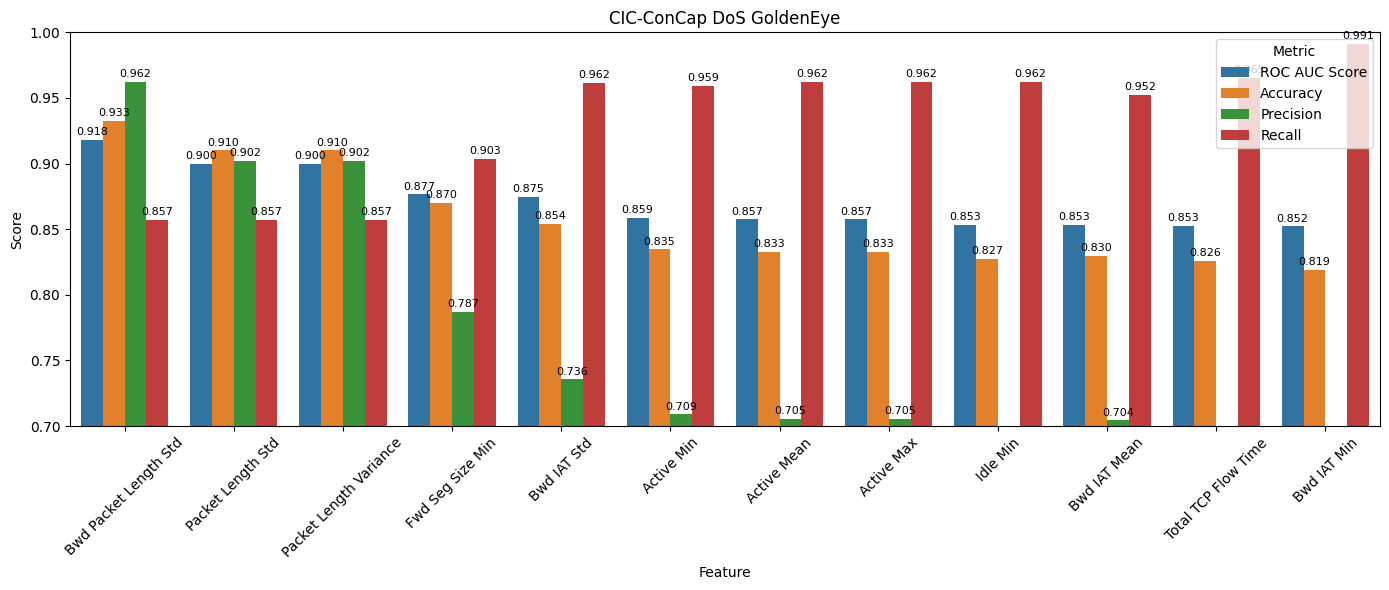
\includegraphics[width=1.2\linewidth]{images/goldeneye_cic_concap}
	\caption{\\Best performing features for DoS GoldenEye when trained on CIC-IDS-2017 traffic and measured on ConCap}
	\label{fig:goldeneye_cic_concap}
\end{figure}
\begin{figure}
	\centering
	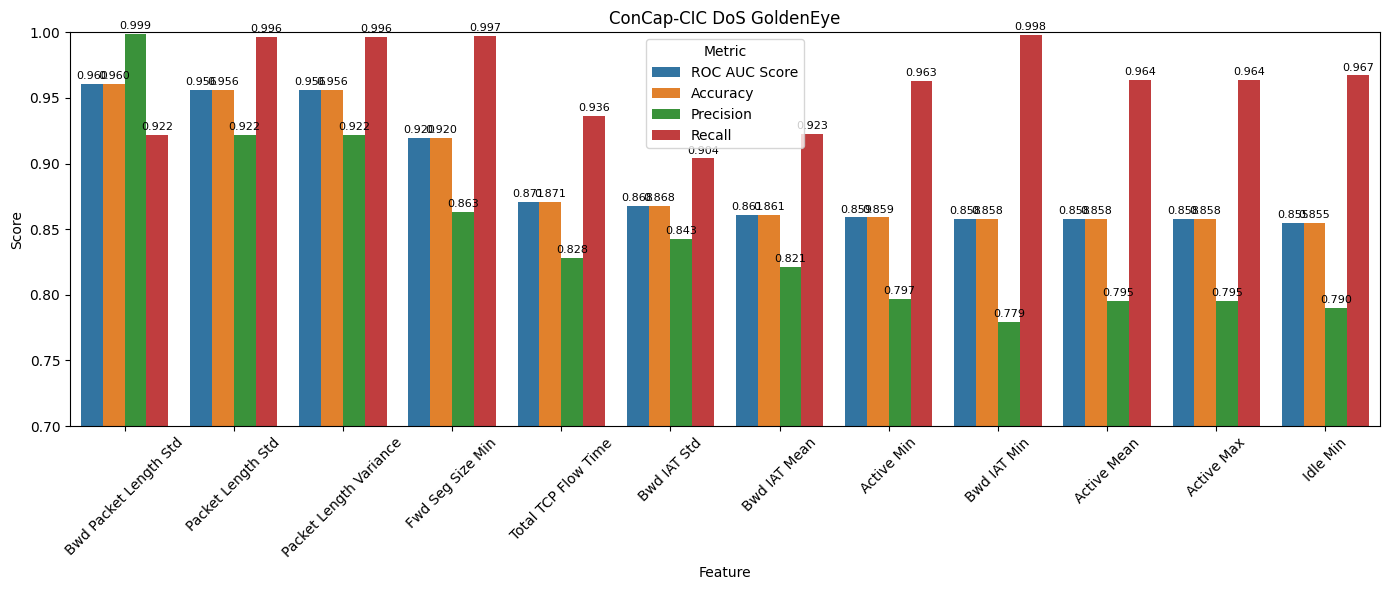
\includegraphics[width=1.2\linewidth]{images/goldeneye_concap_cic}
	\caption{\\Best performing features for DoS GoldenEye when trained on ConCap traffic and measured on CIC-IDS-2017}
	\label{fig:goldeneye_concap_cic}
\end{figure}

\subsubsection{Heartbleed}
For Heartbleed, Figures \ref{fig:heartbleed_cic_concap} and \ref{fig:heartbleed_concap_cic} show only three features scoring above 0.8 ROC AUC Score, with Bwd Packet Length Std being delivering a perfect predictor in both ways of training. We do need to note here that CIC-IDS-2017 has a low amount of Heartbleed flows (11), raising questions about this model's actual performance due to these signs of overfitting. Nevertheless, the best performing features are the three shown, Bwd Packet Length Std (1.000000), Flow Bytes/s (0.931818) and Packet Length Std (0.905702). 

\begin{figure}
	\centering
	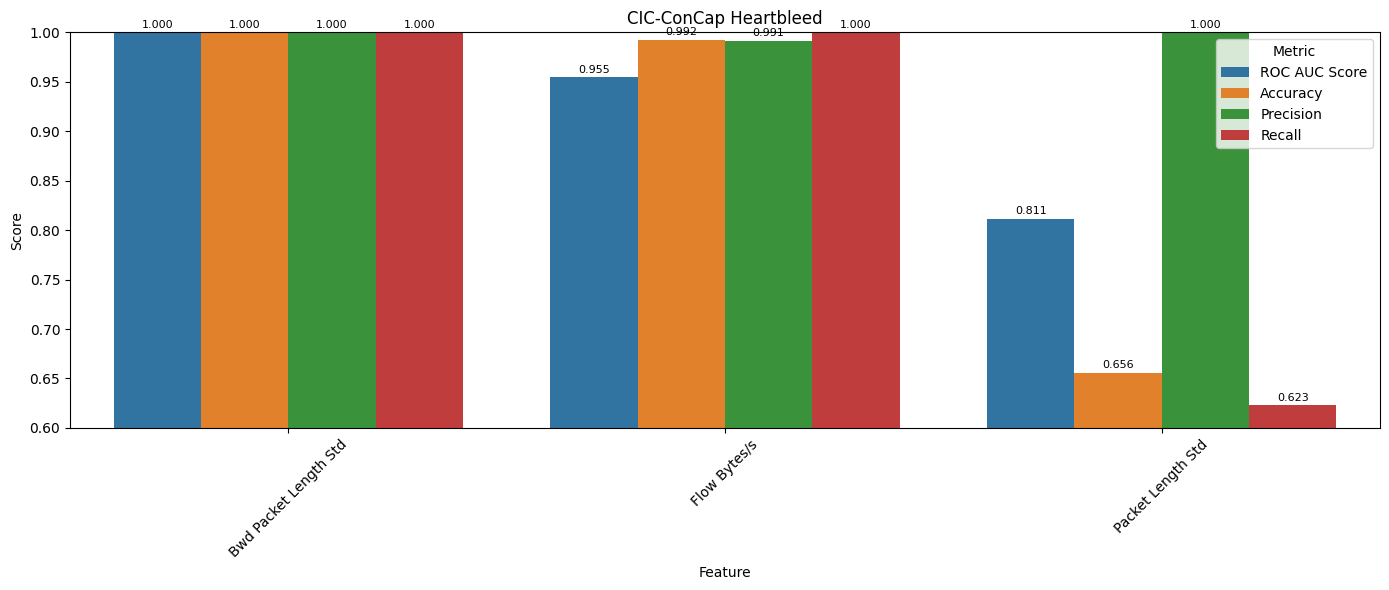
\includegraphics[width=1.2\linewidth]{images/heartbleed_cic_concap}
	\caption{\\Best performing features for Heartbleed bug exploit when trained on CIC-IDS-2017 traffic and measured on ConCap}
	\label{fig:heartbleed_cic_concap}
\end{figure}
\begin{figure}
	\centering
	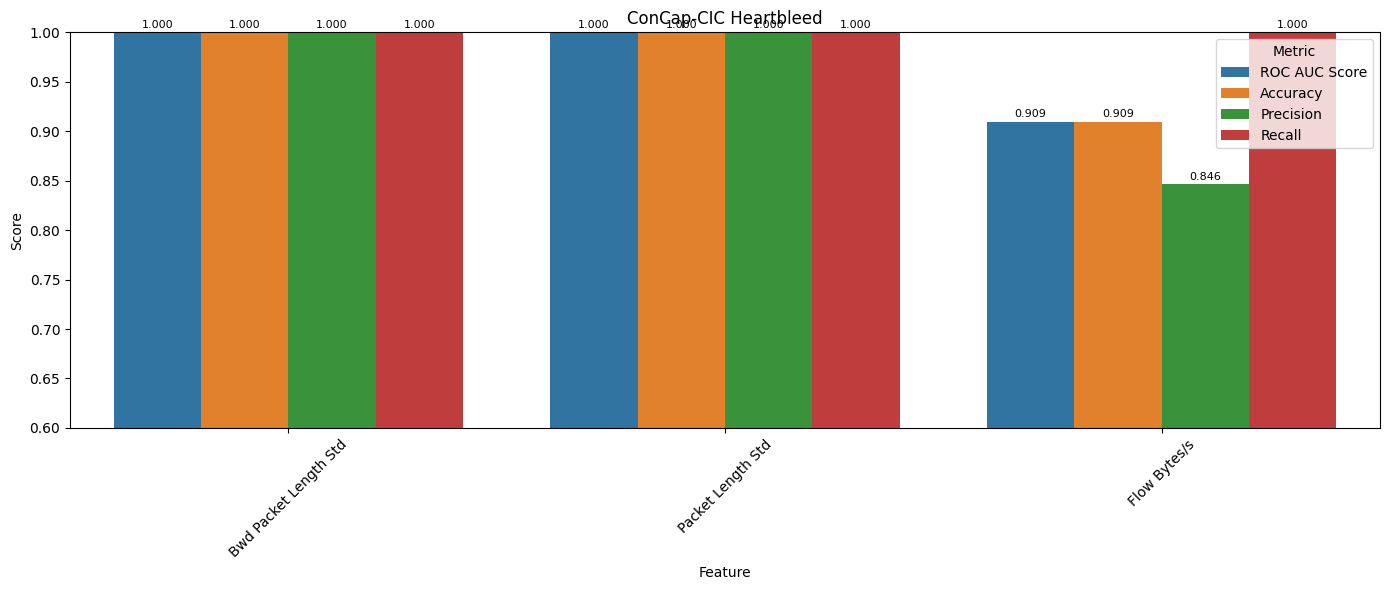
\includegraphics[width=1.2\linewidth]{images/heartbleed_concap_cic}
	\caption{\\Best performing features for Heartbleed bug exploit when trained on ConCap traffic and measured on CIC-IDS-2017}
	\label{fig:heartbleed_concap_cic}
\end{figure}


\subsection{Thursday}

\subsubsection{Web Attacks}
Similarly to Heartbleed, there's only a small number of flows for each of the subcategories of Web Attacks (73, 13 and 18 for Bruteforce, SQL Injection and Cross-Site Scripting respectively). Also similarly we observe features achieving perfect recall, leading us again to suggest that these models are overfitting and not generalizing well. Nevertheless, Figures \ref{fig:web_bruteforce_cic_concap} and \ref{fig:web_bruteforce_concap_cic} show the best performing features of the Bruteforce Web Attack, with best performing features being Fwd Seg Size Min (0.934932), Fwd IAT Min (0.891781) and FIN Flag Count (0.828767).

Figures \ref{fig:web_sqli_cic_concap} and \ref{fig:web_sqli_concap_cic} show the best performing features of SQL Injection attack, with best performing features being Fwd Seg Size Min (0.884615), FIN Flag Count (0.865385) and Bwd IAT Min (0.816719). 

Lastly, Figures \ref{fig:web_xss_cic_concap} and \ref{fig:web_xss_concap_cic} show the best performing features for Cross-Site Scripting attack, with best performing features being Fwd Seg Size Min (0.930556), Bwd Packet Length Std (0.869792) and Packet Length Max (0.845486).

It is clear that Fwd Seg Size Min is the best predictor for the simulated Web Attacks, scoring average ROC AUC score above 0.8 in each category. 

\begin{figure}
	\centering
	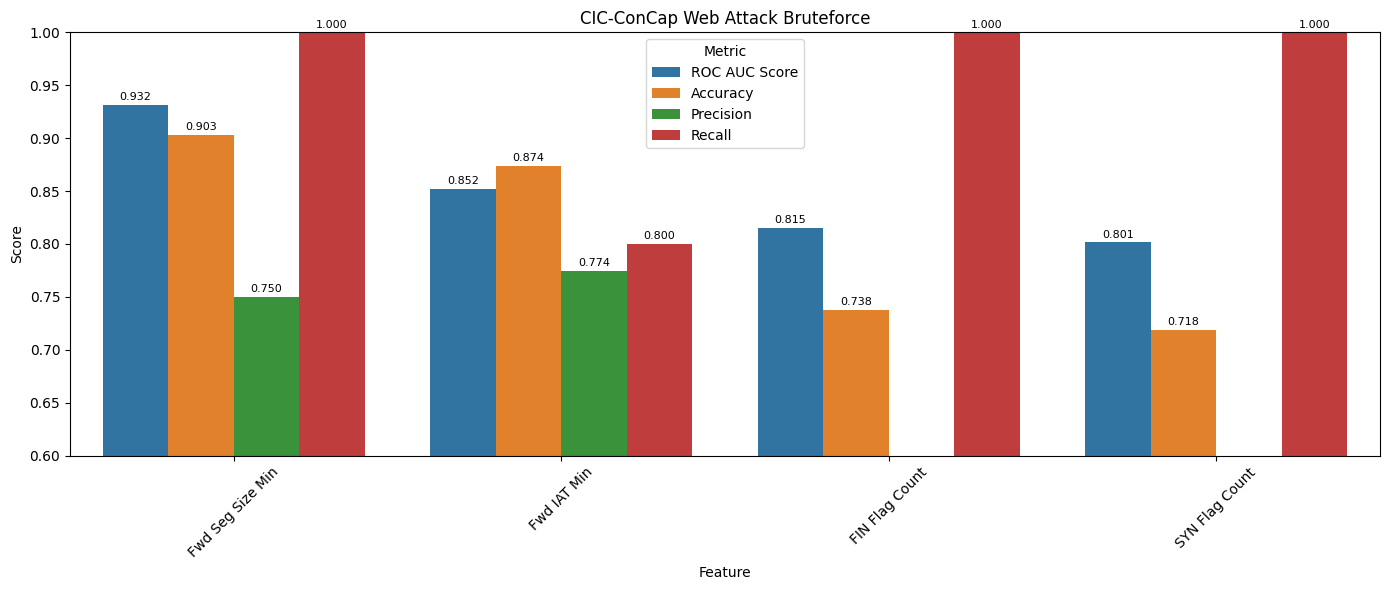
\includegraphics[width=1.2\linewidth]{images/web_bruteforce_cic_concap}
	\caption{\\Best performing features for Bruteforce Web Attack when trained on CIC-IDS-2017 traffic and measured on ConCap}
	\label{fig:web_bruteforce_cic_concap}
\end{figure}
\begin{figure}
	\centering
	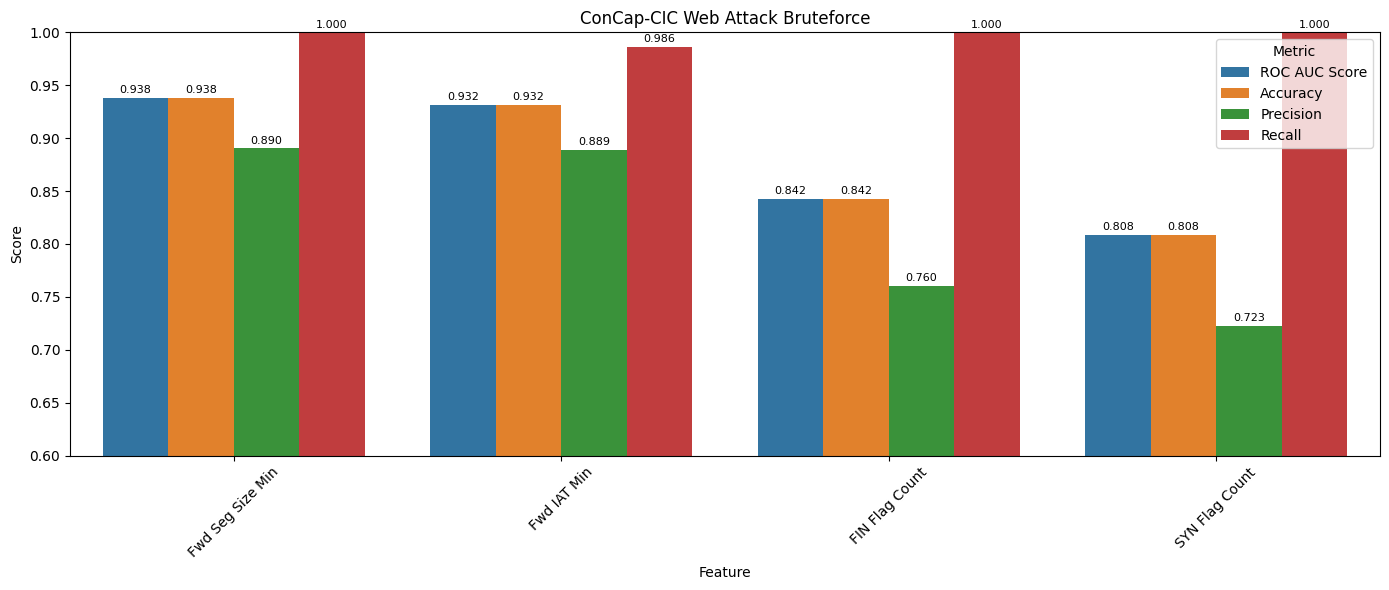
\includegraphics[width=1.2\linewidth]{images/web_bruteforce_concap_cic}
	\caption{\\Best performing features for Bruteforce Web Attack when trained on ConCap traffic and measured on CIC-IDS-2017}
	\label{fig:web_bruteforce_concap_cic}
\end{figure}
\begin{figure}
	\centering
	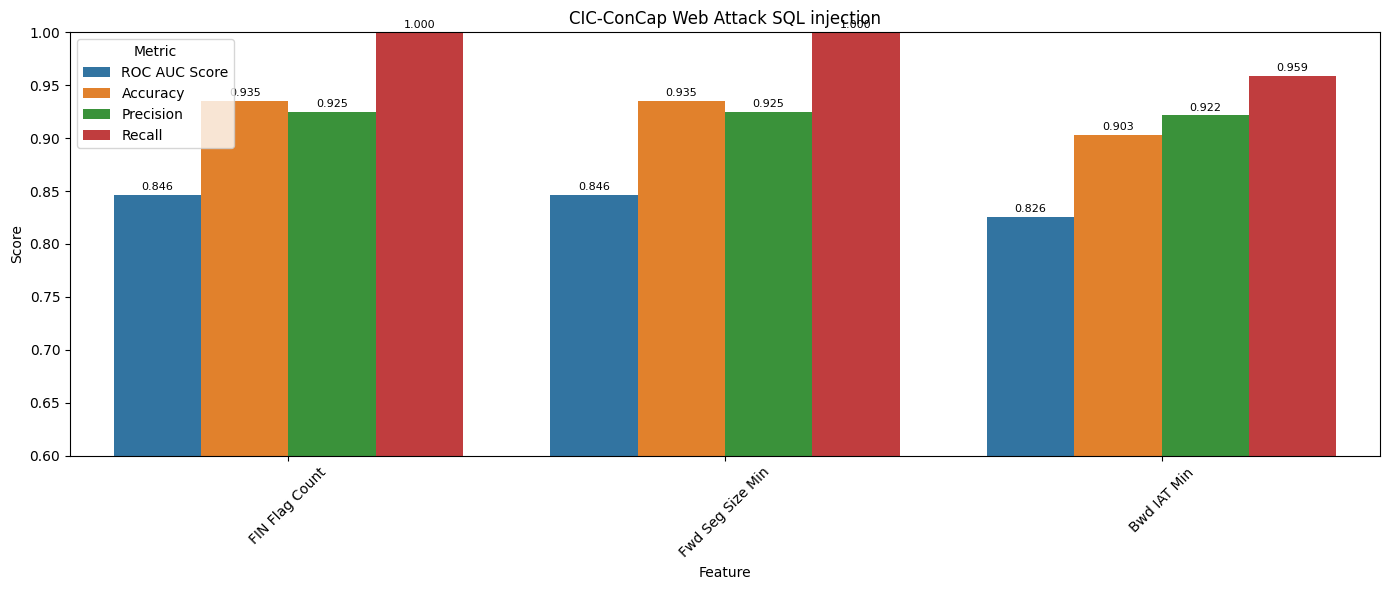
\includegraphics[width=1.2\linewidth]{images/web_sqli_cic_concap}
	\caption{\\Best performing features for SQL Injection Web Attack when trained on CIC-IDS-2017 traffic and measured on ConCap}
	\label{fig:web_sqli_cic_concap}
\end{figure}
\begin{figure}
	\centering
	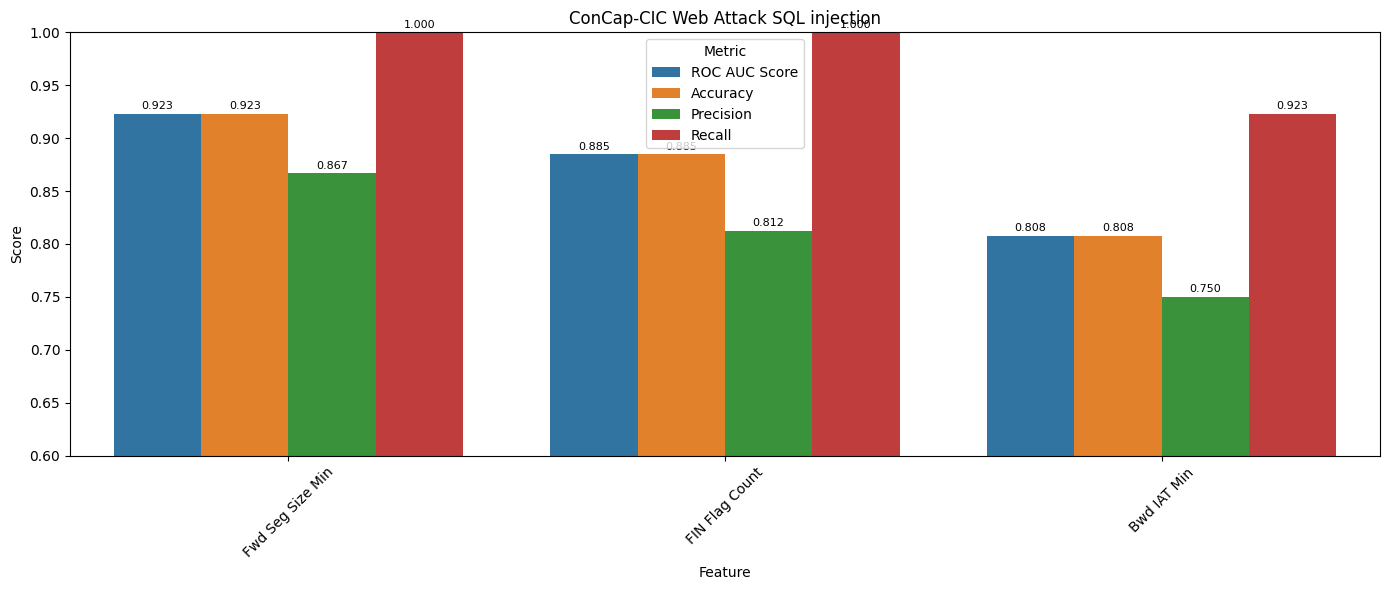
\includegraphics[width=1.2\linewidth]{images/web_sqli_concap_cic}
	\caption{\\Best performing features for SQL Injection Web Attack when trained on ConCap traffic and measured on CIC-IDS-2017}
	\label{fig:web_sqli_concap_cic}
\end{figure}
\begin{figure}
	\centering
	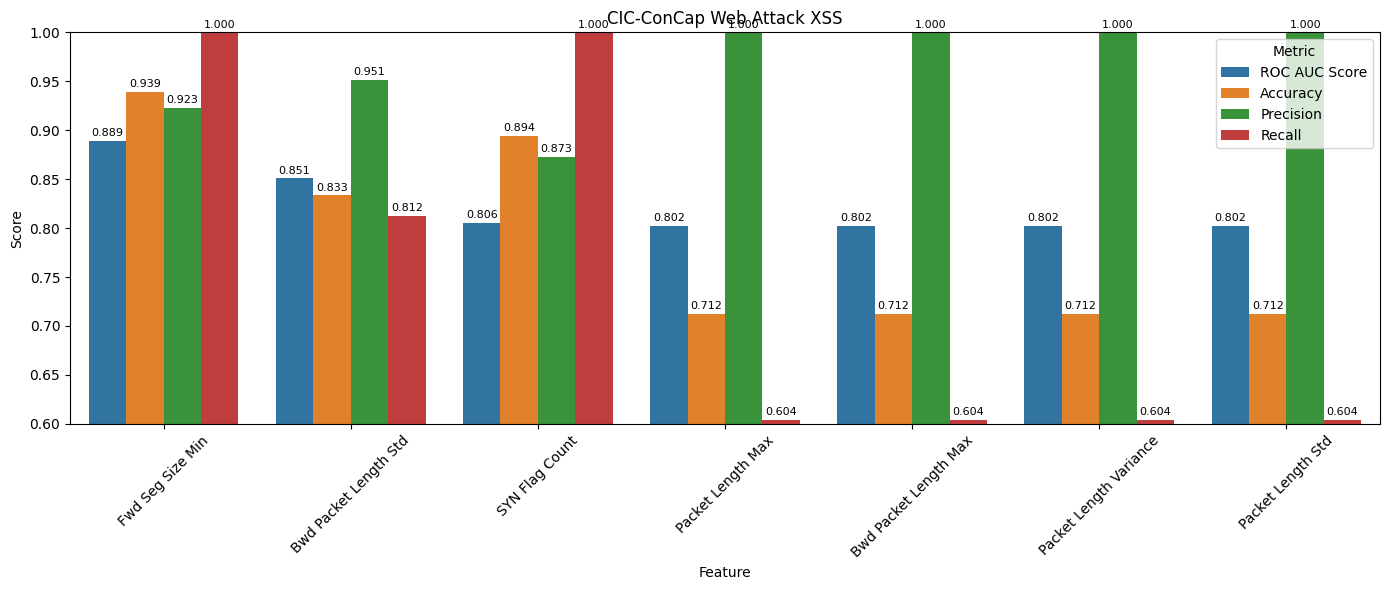
\includegraphics[width=1.2\linewidth]{images/web_xss_cic_concap}
	\caption{\\Best performing features for Cross-Site Scripting Web Attack when trained on CIC-IDS-2017 traffic and measured on ConCap}
	\label{fig:web_xss_cic_concap}
\end{figure}
\begin{figure}
	\centering
	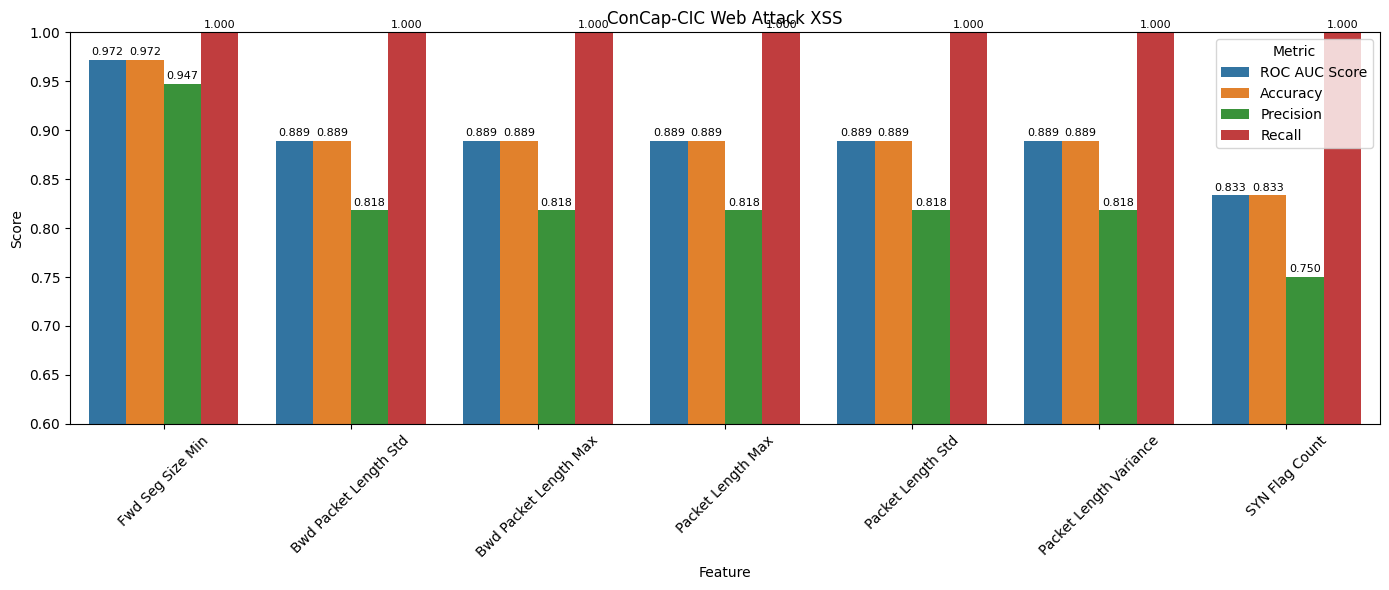
\includegraphics[width=1.2\linewidth]{images/web_xss_concap_cic}
	\caption{\\Best performing features for Cross-Site Scripting Web Attack when trained on ConCap traffic and measured on CIC-IDS-2017}
	\label{fig:web_xss_concap_cic}
\end{figure}

\FloatBarrier

\subsection{Friday}

\subsubsection{LOIC}

For the DDoS LOIC attack, Figures \ref{fig:loic_cic_concap} and \ref{fig:loic_concap_cic} show the focus on features focusing on packet travel time (Fwd IAT Min) as well as opening connections (SYN Flag Count), as we expect given the nature of LOIC being a DDoS tool. The best performing features are Fwd Seg Size Min (0.934932), Fwd IAT Min (0.860959) and FIN Flag Count (0.821918), with SYN Flag Count (0.821918) having the same score as FIN Flag Count.

\begin{figure}
	\centering
	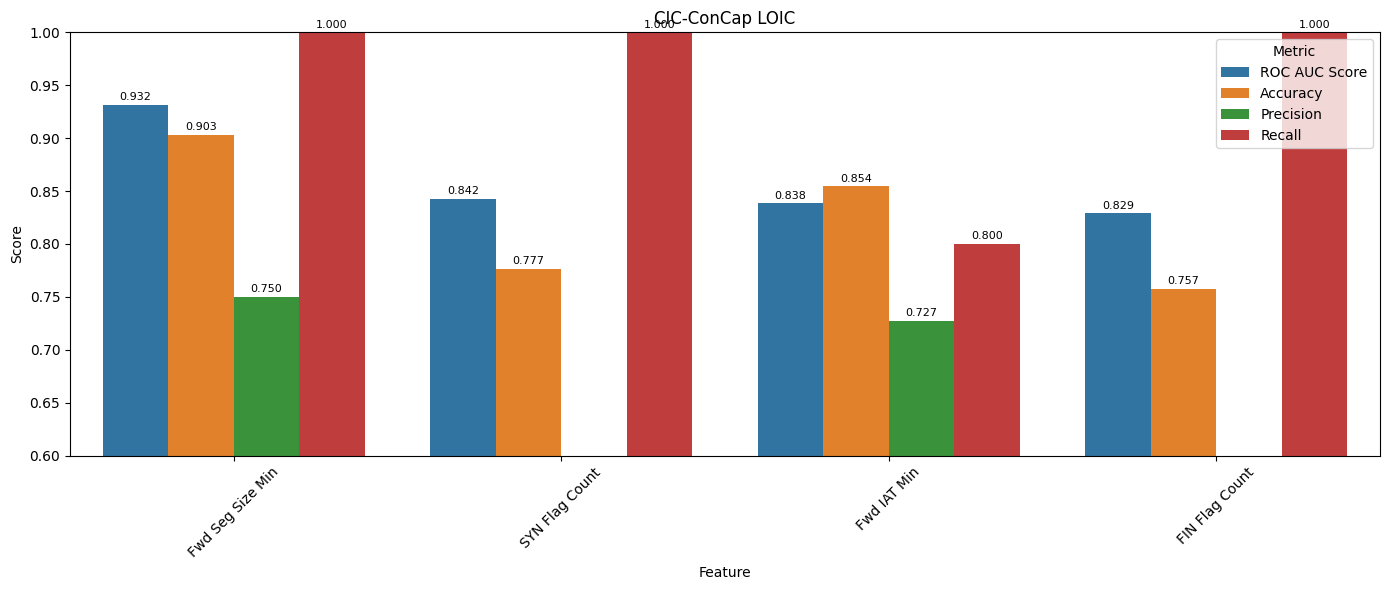
\includegraphics[width=1.2\linewidth]{images/loic_cic_concap}
	\caption{\\Best performing features for DDoS LOIC attack when trained on CIC-IDS-2017 traffic and measured on ConCap}
	\label{fig:loic_cic_concap}
\end{figure}
\begin{figure}
	\centering
	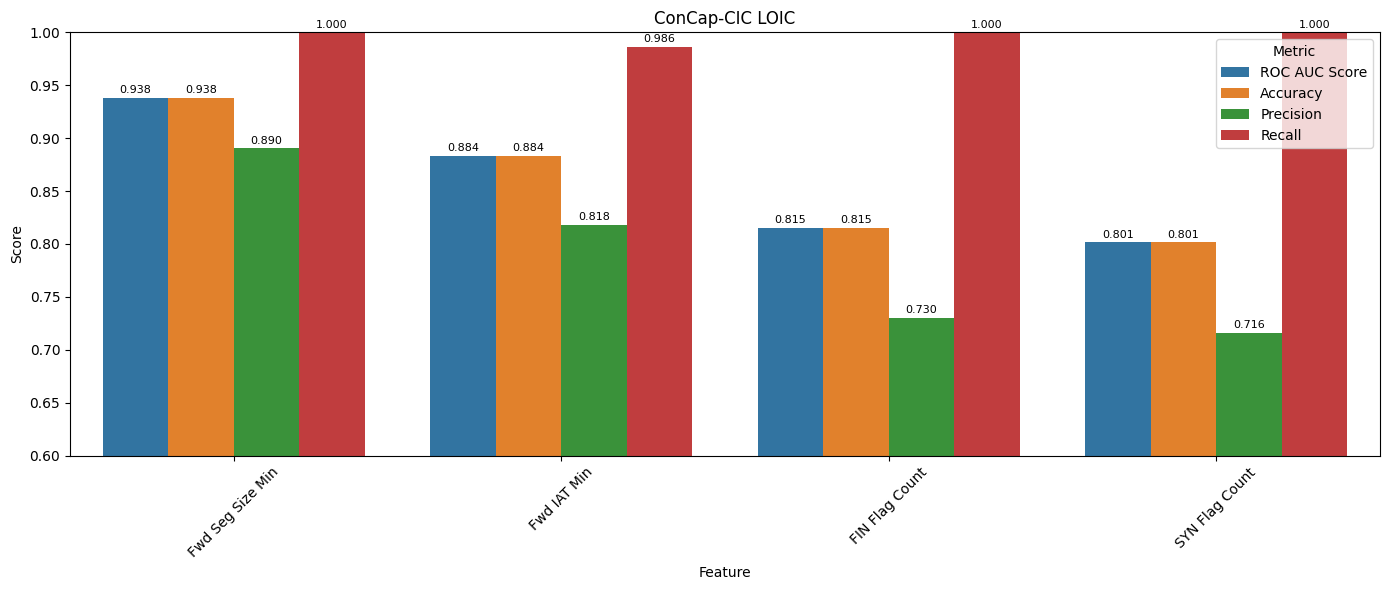
\includegraphics[width=1.2\linewidth]{images/loic_concap_cic}
	\caption{\\Best performing features for DDoS LOIC attack when trained on ConCap traffic and measured on CIC-IDS-2017}
	\label{fig:loic_concap_cic}
\end{figure}

\subsubsection{Portscan}
Finally, Figures \ref{fig:portscan_cic_concap} and \ref{fig:portscan_concap_cic} show the best performing metrics for the Portscan attacks. Noticable is that these attacks are apparently quite easy to classify, given the large amount of metrics that achieve above 0.9 ROC AUC score. Best features appear to be Fwd Packet Length Max (0.949676), Total Length of Fwd Packet (0.948696) and Fwd Segment Size Avg (0.947596). 

\begin{figure}
	\centering
	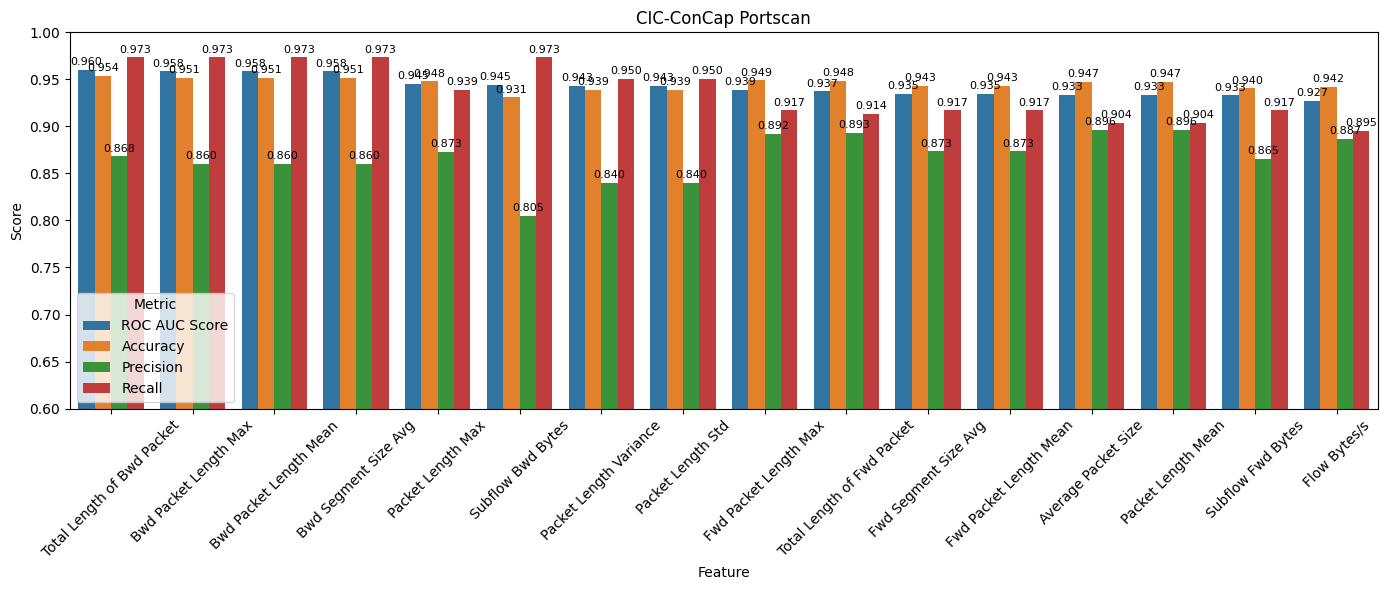
\includegraphics[width=1.2\linewidth]{images/portscan_cic_concap}
	\caption{\\Best performing features for Portscan attack when trained on CIC-IDS-2017 traffic and measured on ConCap}
	\label{fig:portscan_cic_concap}
\end{figure}
\begin{figure}
	\centering
	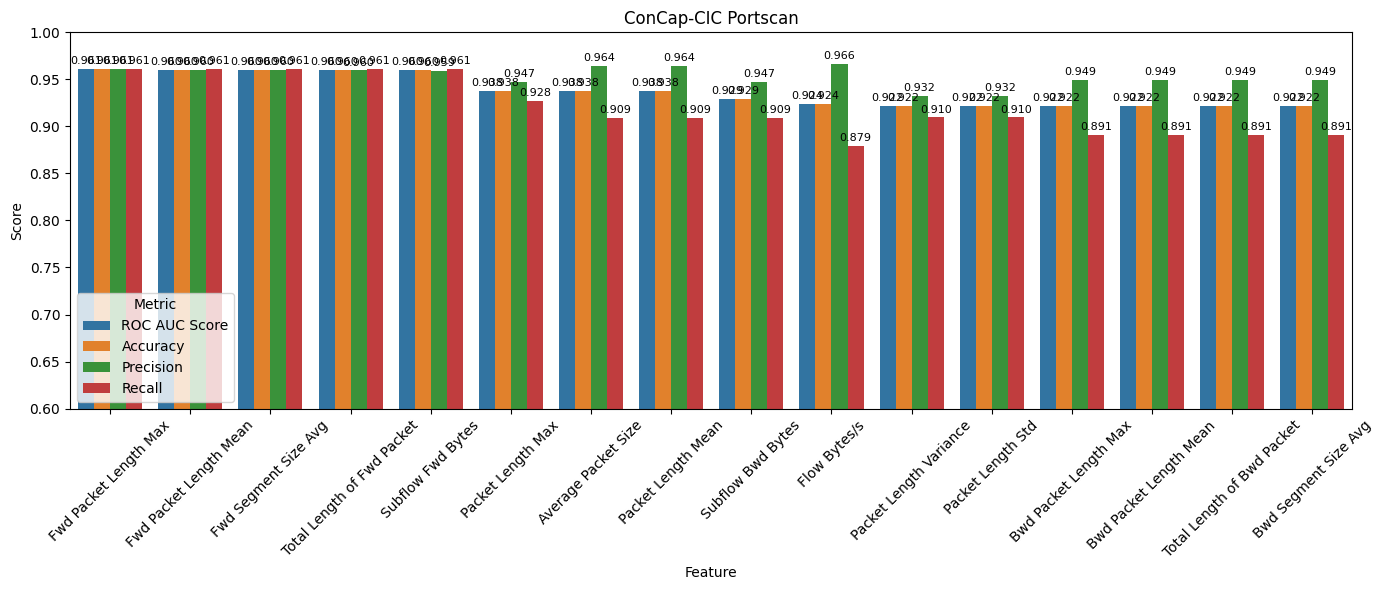
\includegraphics[width=1.2\linewidth]{images/portscan_concap_cic}
	\caption{\\Best performing features for Portscan attack when trained on ConCap traffic and measured on CIC-IDS-2017}
	\label{fig:portscan_concap_cic}
\end{figure}



\newpage
\subsection{Discussion}
The presence and absence of particular features is a peculiar artifact. We speculate that this can be explained by the difference in the methodology of dataset creation. Our reasons for this are threefold. 

First, although ConCap allows for the configuration of network features that affect communication speed, we lack this information about the network conditions of the CIC-IDS-2017 dataset. For this reason, we opt to use the example configuration provided by ConCap authors and keep these conditions the same for all scenarios. Consequently, this could have impact on the prominance of features that are largely determined by the specific network characteristics.

Second, ConCap networks are built fully in-silico and thus do not suffer from the same artifacts as physical networks might: arbitrary delay in packet processing, faulty connections or interference, as well as processing delay. ConCap network architecture is, without introduction of artificial defects, the perfect network. As we lack information about packet drops, reordering or corruptions, we cannot recreate these faithfully, which could have an impact on feature prominance.

Third, the attacks in the CIC-IDS-2017 dataset take place in addition to benign traffic, and the attacks thus form a small minority in the dataset, making it highly imbalanced. We manually balance the training and testing datasets by including known benign flows to achieve class balance. While this should have little effect on features focusing on the size and content of packets (e.g. Packet Length or Flags features), it will have an effect on features that are more concerned with timings (e.g. Flow Bytes/s or Idle features), as the benign flows had no way of influencing attack flows during traffic capture. 

Nevertheless, the results above clearly show presence of features that hold high predictive power for both experiments, leading us to conclude that traffic generated by ConCap can be used instead of the original dataset traffic, as it posesses similar qualities.